The \mf Streamflow Routing (SFR) Package simulates the interactions between surface-water features and groundwater systems. By default, the SFR Package solves a steady, uniform flow equation for each reach under the assumption that flow adjusts instantaneously within each time step. This chapter describes an optional kinematic-wave routing formulation for the SFR Package that accounts for transient storage within stream reaches. The approach is based on the methods described in \cite{McArthur1993} and is equivalent to the ``TRANSROUTE'' option in the SFR Package available in \mfn \citep{modflownwt} and first described in \citet{markstrom2008gsflow}. Accurate representation of flood-wave timing requires that the model time step be comparable to the kinematic-wave travel time through a reach; guidance for selecting the time step is provided in the Practical Guidance section.

\subsection{Kinematic-Wave Approximation}

The one-dimensional Saint-Venant equations for open-channel flow combine the continuity equation and the momentum equation. The momentum equation includes terms representing local acceleration, advective acceleration, pressure gradient, gravity, and friction. The kinematic-wave approximation retains only the gravity and friction terms in the momentum equation, which is equivalent to assuming that the energy grade line is parallel to the channel bed slope. Under this approximation, the discharge $Q$ ($L^3T^{-1}$) is uniquely determined by the depth of flow and the channel geometry, and the governing equation reduces to the continuity equation alone \citep{LighthillWhitham1955, PonceSimons1977, PonceLiSimons1978}

\begin{equation}
	\label{eqn:sfr-continuity}
	\frac{\partial Q}{\partial x} + \frac{\partial A}{\partial t} = q_L ,
\end{equation}

\noindent where $Q$ is the volumetric discharge ($L^3T^{-1}$); $A$ is the cross-sectional area of flow ($L^2$); $x$ is the longitudinal distance along the channel ($L$); $t$ is time ($T$); and $q_L$ is the lateral inflow rate per unit channel length ($L^2T^{-1}$). The kinematic-wave approximation is applicable when the channel slope is sufficiently steep relative to the backwater effect and the Froude number is less than about 2, above which roll waves can develop and the kinematic wave no longer approximates the dynamic wave \citep{McArthur1993, WoolhiserLiggett1967, PonceLiSimons1978, Ponce1991}.

The discharge in a reach is calculated using Manning's equation \citep{Manning1891}

\begin{equation}
	\label{eqn:sfr-manning}
	Q = \frac{\alpha}{n} A R^{2/3} S_0^{1/2} ,
\end{equation}

\noindent where $\alpha$ is a unit conversion factor ($\alpha = 1$ for SI units; $\alpha = 1.486$ for U.S.~customary units); $n$ is Manning's roughness coefficient ($TL^{-1/3}$); $R$ is the hydraulic radius ($L$) defined as $R = A / P_w$ where $P_w$ is the wetted perimeter ($L$); and $S_0$ is the channel bed slope (dimensionless). Equation~\ref{eqn:sfr-manning} establishes a nonlinear, monotonically increasing relationship between $Q$ and $A$ (or equivalently, between $Q$ and flow depth $d$) for a given channel geometry. This functional relationship is used to determine the depth corresponding to a computed discharge and to evaluate the wet cross-sectional area \citep{chaudhry2008}.

The kinematic-wave celerity $c$ ($LT^{-1}$) is the speed at which a perturbation (a flood peak) propagates downstream. It is defined as the derivative of discharge with respect to cross-sectional area

\begin{equation}
	\label{eqn:sfr-celerity}
	c = \frac{dQ}{dA} .
\end{equation}

\noindent In practice, the celerity is evaluated numerically by finite difference as

\begin{equation}
	\label{eqn:sfr-celerity-num}
	c \approx \frac{\delta}{A(Q + \delta) - A(Q)} ,
\end{equation}

\noindent where $\delta$ is a small perturbation in discharge and $A(Q)$ is the cross-sectional area corresponding to discharge $Q$, obtained by inverting Manning's equation (eq.~\ref{eqn:sfr-manning}). For a Manning's-equation-based channel, the kinematic-wave celerity is approximately $5/3$ times the mean flow velocity at low depths and may be several times the mean velocity in wide channels \citep{LighthillWhitham1955, chaudhry2008}.

The Courant number $C_r$ (dimensionless) relates the wave celerity to the computational cell size

\begin{equation}
	\label{eqn:sfr-courant}
	C_r = \frac{c \, \Delta t}{\Delta x} ,
\end{equation}

\noindent where $\Delta t$ is the time step length ($T$) and $\Delta x$ is the reach length ($L$). The Courant number governs the temporal weighting used in the finite-difference approximation of equation~\ref{eqn:sfr-continuity}.

\subsection{Finite-Difference Discretization}

A four-point implicit finite-difference scheme \citep{Preissmann1961} is used to discretize equation~\ref{eqn:sfr-continuity} on each reach. The scheme uses the upstream and downstream flow values at both the current and previous time steps, as illustrated in figure~\ref{fig:sfr-stencil}. In the SFR implementation, the four nodal discharges are referred to as $Q_a$, $Q_b$, $Q_c$, and $Q_d$: $Q_a = Q_U^{n-1}$ and $Q_b = Q_D^{n-1}$ are the upstream and downstream discharge at the previous time step; $Q_c = Q_U^n$ is the upstream discharge at the current time step (known from the reach inflow); and $Q_d = Q_D^n$ is the downstream discharge at the current time step (the unknown to be determined). The corresponding cross-sectional areas are $A_a$, $A_b$, $A_c$, and $A_d$.

\begin{figure}[!ht]
	\begin{center}
	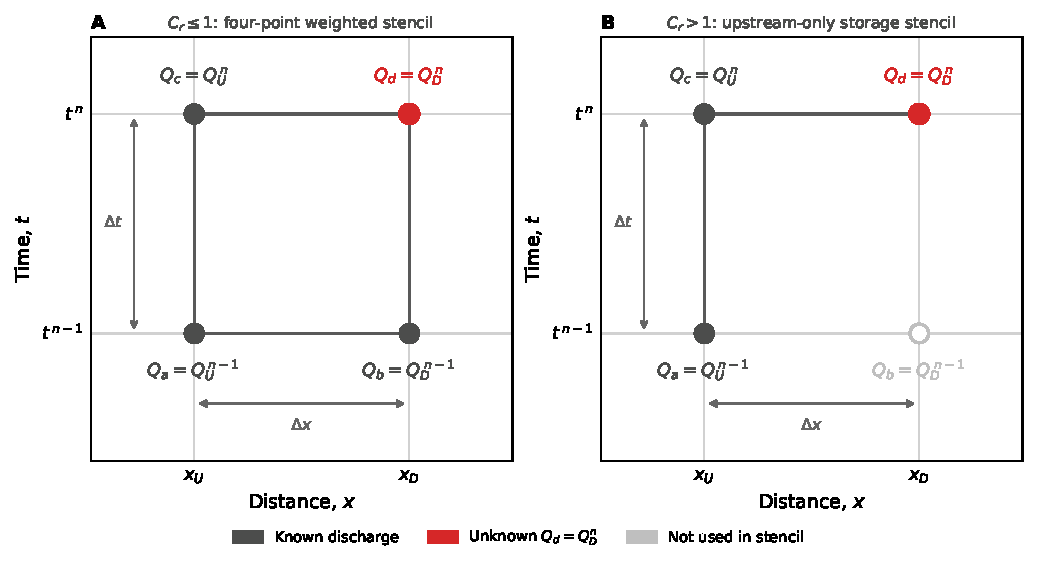
\includegraphics{./Figures/SFRKinematicWaveStencil.pdf}
	\caption[Space-time grid diagrams for the kinematic-wave finite-difference stencils used in the \mf SFR Package]{Space-time grid diagrams showing the nodal positions and variable names for the two kinematic-wave finite-difference stencils used in the \mf SFR Package ($Q_a = Q_U^{n-1}$, $Q_b = Q_D^{n-1}$, $Q_c = Q_U^n$, $Q_d = Q_D^n$). Filled nodes are known values; the red node ($Q_d$) is the unknown. \textit{A}, When $C_r \le 1$, all four nodes participate in the spatial and temporal difference approximations; \textit{B}, when $C_r > 1$, only the upstream temporal difference is retained for the storage term (the $Q_b$ node is not used)}
	\label{fig:sfr-stencil}
	\end{center}
\end{figure}

In the Preissmann scheme, the spatial derivative $\partial Q / \partial x$ is approximated at the temporal mid-point of the stencil as a weighted average of the spatial gradients at the two time levels, and the temporal derivative $\partial A / \partial t$ is approximated at the spatial mid-point as the average of the area changes at the two end nodes. Two discretizations arise depending on whether the Courant number is above or below unity.

When $C_r \le 1$, the scheme applies a temporal weighting parameter $\theta$ ($0.5 \le \theta \le 1$) to the spatial gradient term and averages the storage change over both time levels

\begin{equation}
	\label{eqn:sfr-residual-low-cr}
	\frac{\theta \left( Q_D^n - Q_U^n \right) + \left(1 - \theta \right) \left( Q_D^{n-1} - Q_U^{n-1} \right)}{\Delta x}
	+ \frac{1}{2} \frac{\left( A_D^n - A_D^{n-1} \right) + \left( A_U^n - A_U^{n-1} \right)}{\Delta t} = q_L ,
\end{equation}

\noindent where $q_L$ is the net lateral inflow per unit length at the current time step ($L^2T^{-1}$), including contributions from overland runoff, evaporation, precipitation, and groundwater exchange. When $\theta = 1$, the scheme reduces to a fully implicit, first-order accurate spatial discretization. When $\theta = 0.5$, the scheme is second-order accurate in time and is equivalent to the Crank-Nicolson approximation.

When $C_r > 1$, the scheme uses only the current time step values at the upstream node for the storage term, which prevents the introduction of numerical instabilities that can arise when the wave speed exceeds the Courant stability limit for the $C_r \le 1$ scheme

\begin{equation}
	\label{eqn:sfr-residual-high-cr}
	\frac{Q_D^n - Q_U^n}{\Delta x} + \frac{A_U^n - A_U^{n-1}}{\Delta t} = q_L .
\end{equation}

\noindent Under this condition, the kinematic-wave crest has already propagated through the entire reach within a single time step. Because the previous-time-level downstream state ($Q_D^{n-1}$, $A_D^{n-1}$) carries no information about the current wave front, it is excluded from the difference approximations; only the upstream area change $A_U^n - A_U^{n-1}$ captures the wave's passage through the reach.

The two cases may be written as a single residual function $f(Q_D^n)$

\begin{equation}
	\label{eqn:sfr-residual}
	f \left( Q_D^n \right) = \frac{\partial Q}{\partial x}\bigg|_\mathrm{fd} + \frac{\partial A}{\partial t}\bigg|_\mathrm{fd} - q_L = 0 ,
\end{equation}

\noindent where the finite-difference approximations correspond to equations~\ref{eqn:sfr-residual-low-cr} or \ref{eqn:sfr-residual-high-cr} depending on the Courant number. The unknown $Q_D^n$ enters through both the discharge term and the area term (because $A_D^n$ is determined from $Q_D^n$ via Manning's equation). Equation~\ref{eqn:sfr-residual} is solved iteratively using a Newton-Raphson method

\begin{equation}
	\label{eqn:sfr-newton}
	Q_D^{n, k+1} = Q_D^{n, k} - \frac{f \left( Q_D^{n, k} \right)}{f' \left( Q_D^{n, k} \right)} ,
\end{equation}

\noindent where the superscript $k$ denotes the Newton-Raphson iteration index and $f'$ is the derivative of the residual with respect to $Q_D^n$, approximated numerically.

The change in water stored within a reach during a time step is required to ensure conservation of mass in the water budget. The storage change $\Delta S$ ($L^3T^{-1}$) is calculated from the cross-sectional area values at the upstream and downstream ends of the reach at both time levels. For $C_r \le 1$

\begin{equation}
	\label{eqn:sfr-storage-low-cr}
	\Delta S = \frac{1}{2} \left[ \left( A_U^n + A_D^n \right) - \left( A_U^{n-1} + A_D^{n-1} \right) \right] \frac{\Delta x}{\Delta t} ,
\end{equation}

\noindent and for $C_r > 1$

\begin{equation}
	\label{eqn:sfr-storage-high-cr}
	\Delta S = \left( A_U^{n-1} - A_U^n \right) \frac{\Delta x}{\Delta t} .
\end{equation}

\noindent For $C_r \le 1$, the storage change is estimated from the trapezoidal average of the areas at both ends of the reach at both time levels. For $C_r > 1$, only the upstream area change is used, consistent with the assumption that the wave has already propagated through the reach. Note that the area differences in equations~\ref{eqn:sfr-storage-low-cr} and \ref{eqn:sfr-storage-high-cr} are the same terms that appear in the finite-difference residual (eqs.~\ref{eqn:sfr-residual-low-cr} and \ref{eqn:sfr-residual-high-cr}); the residual enforces continuity during the Newton-Raphson solve, while $\Delta S$ is computed separately once convergence is reached for use in the reach water budget. The appropriate expression is selected automatically based on the Courant number evaluated at each reach and time step. Equation~\ref{eqn:sfr-mf6-storage} provides the equivalent form as implemented in \mf, evaluated using the converged areas after Newton-Raphson convergence.

\subsection{Implementation in \mf}

The kinematic-wave routing option is activated by specifying the \texttt{STORAGE} keyword in the OPTIONS block of the SFR Package input file \citep{modflow6gwf}. When \texttt{STORAGE} is activated, the SFR Package allocates storage for the upstream and downstream flow values from the previous time step and solves equation~\ref{eqn:sfr-residual} at each reach and time step using a Picard outer loop that also couples stream-aquifer exchange. The Picard loop iterates until the change in average reach depth (mean of upstream and downstream depths) falls below the \texttt{MAXIMUM\_DEPTH\_CHANGE} parameter (default $1 \times 10^{-5}$~m); for reaches with no groundwater exchange, the coupling is one-way and the loop reduces to a single iteration. The \texttt{MAXIMUM\_DEPTH\_CHANGE} parameter is package-wide and also controls the convergence tolerance for the standard instantaneous-flow formulation during steady-state stress periods. The kinematic-wave routing option in \mf was validated against the modified Pinder-Sauer problem \citep{pinder1971numerical, lal2001modification}, which describes flood-wave attenuation due to bank storage effects and provides an analytical solution for stream-aquifer interaction under transient conditions.

\subsubsection{Standard Kinematic-Wave Scheme}

The standard kinematic-wave scheme solves for the unknown downstream discharge $Q_D^n$ at each reach by finding the root of the finite-difference residual using Newton-Raphson iteration. The lateral source term $q_L$ in the residual aggregates all per-reach inflow and loss contributions, and the temporal weighting parameter $\theta$ controls the balance between numerical stability and temporal accuracy. Once the Newton-Raphson iteration has converged, the volumetric storage change is computed explicitly from the converged cross-sectional areas to close the reach water budget.

The net lateral source per unit length, $q_L$ ($L^2T^{-1}$), combines all per-reach inflow and loss terms

\begin{equation}
	\label{eqn:sfr-qlat}
	q_L = \frac{q_r + q_{ro} - q_e}{\Delta x} - \frac{q_{gwf}}{\Delta x} ,
\end{equation}

\noindent where $q_r$ is direct precipitation onto the reach ($L^3T^{-1}$); $q_{ro}$ is overland runoff into the reach ($L^3T^{-1}$); $q_e$ is evaporation from the reach ($L^3T^{-1}$); and $q_{gwf}$ is the groundwater exchange flux ($L^3T^{-1}$, positive out of the stream). Inflow specified with the \texttt{INFLOW} keyword and water provided by the Water Mover (MVR) Package are not part of $q_L$. Both are volumetric rates ($L^3T^{-1}$) delivered to the reach rather than sources distributed along it, and are added to the upstream discharge $Q_U^n$ together with flow from connected upstream reaches. Dividing by $\Delta x$ converts these volumetric fluxes to the per-unit-length form required by equation~\ref{eqn:sfr-continuity}. All terms are evaluated at the current Picard iteration.

The temporal weighting parameter $\theta$ defaults to 1.0 (fully implicit). Values of $\theta$ between 0.5 and 1.0 are accepted; values less than 0.5 are not permitted because they can produce unstable solutions. A value of $\theta = 1.0$ provides maximum numerical stability at the cost of first-order temporal accuracy and is strongly recommended for all practical applications. When $\theta = 0.5$, equation~\ref{eqn:sfr-mf6-residual} becomes the Crank-Nicolson scheme \citep{CrankNicolson1947}, which is second-order accurate in time but may exhibit oscillations when $C_r < 1$ and the spatial discretization is coarse. The Courant number is evaluated at each reach and time step using the celerity estimated from the effective upstream inflow---the upstream discharge $Q_U^n$ adjusted for lateral contributions and groundwater exchange (eq.~\ref{eqn:sfr-courant}).

The finite-difference residual for each reach is evaluated at each Newton-Raphson iteration $k$ as

\begin{equation}
	\label{eqn:sfr-mf6-residual}
	f\!\left(Q_D^{n,k}\right) =
	\begin{dcases}
		\begin{aligned}
			&\dfrac{\theta \left(Q_D^{n,k} - Q_U^n\right) + \left(1-\theta\right)\!\left(Q_D^{n-1} - Q_U^{n-1}\right)}{\Delta x} \\[4pt]
			&\quad + \dfrac{\left(A_D^{n,k} - A_D^{n-1}\right) + \left(A_U^n - A_U^{n-1}\right)}{2\,\Delta t} - q_L
		\end{aligned}
		& C_r \le 1 \\[12pt]
		\dfrac{Q_D^{n,k} - Q_U^n}{\Delta x}
		+ \dfrac{A_U^n - A_U^{n-1}}{\Delta t} - q_L
		& C_r > 1
	\end{dcases} ,
\end{equation}

\noindent where $A_D^{n,k}$ is the wet cross-sectional area at the downstream end corresponding to $Q_D^{n,k}$, evaluated by inverting Manning's equation (eq.~\ref{eqn:sfr-manning}).

Because the area $A_D^{n,k}$ depends nonlinearly on $Q_D^{n,k}$, equation~\ref{eqn:sfr-mf6-residual} is nonlinear and is solved with Newton-Raphson iteration, starting from the initial guess $Q_D^{n,0} = Q_D^{n-1}$ (the downstream discharge from the previous time step); when $Q_D^{n-1} = 0$---for example, at the start of a transient simulation or after a reach has gone dry---the initial guess is taken as $\tfrac{1}{2}(Q_U^n + Q_D^{n-1})$ instead. The derivative $f'$ is approximated by a forward finite difference using a small discharge perturbation $\delta$

\begin{equation}
	\label{eqn:sfr-mf6-deriv}
	f'\!\left(Q_D^{n,k}\right) \approx \frac{f\!\left(Q_D^{n,k} + \delta\right) - f\!\left(Q_D^{n,k}\right)}{\delta} ,
\end{equation}

\noindent and the discharge is updated as

\begin{equation}
	\label{eqn:sfr-mf6-update}
	Q_D^{n,k+1} = Q_D^{n,k} - \frac{f\!\left(Q_D^{n,k}\right)}{f'\!\left(Q_D^{n,k}\right)} .
\end{equation}

\noindent The updated discharge is limited to a minimum of $10^{-30}$~m$^3$\,s$^{-1}$ to keep it positive. Iteration continues until

\begin{equation}
	\label{eqn:sfr-mf6-converge}
	\left| Q_D^{n,k+1} - Q_D^{n,k} \right| < 2\delta
	\quad \text{and} \quad
	\left| f\!\left(Q_D^{n,k+1}\right) \right| < 2\delta ,
\end{equation}

\noindent or until the maximum of 100 Newton-Raphson iterations is reached. The perturbation $\delta$ is set to $0.999 \times \texttt{MAXIMUM\_DEPTH\_CHANGE}$ and is used for the numerical celerity estimate (eq.~\ref{eqn:sfr-celerity-num}), the numerical derivative (eq.~\ref{eqn:sfr-mf6-deriv}), and the Newton-Raphson convergence test (eq.~\ref{eqn:sfr-mf6-converge}). The Picard depth-change tolerance equals \texttt{MAXIMUM\_DEPTH\_CHANGE} directly. Both are governed by the same input parameter.

A dry reach that gains water from the aquifer---where the aquifer head lies above the streambed top---but receives little or no inflow from upstream cannot rewet with the standard iterative solution: at zero depth both the wetted cross-sectional area and the streambed conductance vanish, so a dry reach stays dry and receives no groundwater discharge. To overcome this issue, the depth in dry reaches that receive groundwater discharge is instead found by bisection between a small wet depth and the aquifer depth above the streambed top, which lets the reach rewet and receive groundwater discharge for any time-step size. Reaches that receive meaningful inflow from upstream are solved with the standard iteration approach.

After Newton-Raphson convergence, the volumetric storage change $\Delta S$ ($L^3T^{-1}$) for the reach water budget is computed from equations~\ref{eqn:sfr-storage-low-cr} and \ref{eqn:sfr-storage-high-cr} using the converged areas

\begin{equation}
	\label{eqn:sfr-mf6-storage}
	\Delta S =
	\begin{dcases}
		\dfrac{1}{2}\left[\left(A_U^n + A_D^n\right) - \left(A_U^{n-1} + A_D^{n-1}\right)\right] \dfrac{\Delta x}{\Delta t}
		& C_r \le 1 \\[10pt]
		\left(A_U^{n-1} - A_U^n\right) \dfrac{\Delta x}{\Delta t}
		& C_r > 1
	\end{dcases} .
\end{equation}

\subsubsection{TVD Kinematic-Wave Routing}
\label{sec:sfr-tvd}

An alternative explicit routing scheme based on a Total Variation Diminishing (TVD) finite-volume discretization is activated by specifying the \texttt{ATS\_COURANT} parameter in the OPTIONS block of the SFR Package. The TVD scheme replaces the Newton-Raphson iteration of the standard kinematic-wave scheme with a direct, one-step volume balance that guarantees exact mass conservation at every reach and every time step, independent of convergence tolerance \citep{Harten1983, LeVeque2002}. The standard scheme closes the budget to within the Newton-Raphson convergence tolerance, which is negligible for the default \texttt{MAXIMUM\_DEPTH\_CHANGE} $= 10^{-5}$~m but can become measurable on steep wave fronts or during dry-reach transitions.

The TVD scheme is most appropriate when exact mass conservation is required---for example, when simulated streamflow will be used as input to a solute transport model. Because the explicit TVD formulation is conditionally stable only for $C_r \le 1$, targeting $C_r \approx 1$ fixes the time step at approximately $\Delta t \approx \Delta x / c$. For typical reach lengths and flow conditions this implies sub-daily time steps (e.g., $\Delta t \approx$ 400--1,000~s for 500-m reaches at moderate base flows), which may be substantially shorter than the time steps used in the groundwater model. The standard kinematic-wave scheme is sufficient for most stream-routing applications and accommodates Courant numbers from about 0.5 to 2 without such strict time-step constraints.

\paragraph{TVD Scheme Formulation}

The TVD scheme avoids iterating on a residual equation; instead it updates each reach directly with an explicit volume balance. At each time step the scheme operates as follows.

\textit{Step 1---First-order upwind flux.}
The outflow flux at the previous time level is estimated from Manning's equation (eq.~\ref{eqn:sfr-manning}) evaluated at the stored reach depth $d^{n-1}$

\begin{equation}
  \label{eqn:sfr-tvd-upwind}
  q_\mathrm{out}^{n-1} = Q_\mathrm{Manning}\!\left(d^{n-1}\right) .
\end{equation}

\noindent Using the stored depth rather than a previous-step discharge variable ensures that the upwind flux reflects the actual water volume in the reach, which is critical for correct dry-reach wetting behavior.

\textit{Step 2---Van Leer anti-diffusion correction.}
When a reach has a single identified upstream neighbor (index $i_\mathrm{up}$), a second-order Lax-Wendroff correction is applied and bounded by the van Leer flux limiter \citep{vanLeer1974}

\begin{equation}
  \label{eqn:sfr-tvd-vanleer}
  q_\mathrm{TVD} = q_\mathrm{out}^{n-1}
    + \frac{1}{2}(1 - C_r)\,\phi(r)\,\Delta q_\mathrm{loc} ,
\end{equation}

\noindent where $\Delta q_\mathrm{loc} = q_\mathrm{out}^{n-1} - q_{U}^{n-1}$ is the local flow gradient, $\Delta q_\mathrm{up} = q_{U}^{n-1} - q_{U_2}^{n-1}$ is the upstream flow gradient ($q_{U}^{n-1}$ and $q_{U_2}^{n-1}$ are the inflows from the immediate and second upstream reaches), $r = \Delta q_\mathrm{up} / \Delta q_\mathrm{loc}$ is the ratio of upstream to local gradient, and $\phi(r)$ is the van Leer flux limiter

\begin{equation}
  \label{eqn:sfr-tvd-limiter}
  \phi(r) = \frac{r + |r|}{1 + |r|} .
\end{equation}

\noindent The limiter satisfies the TVD condition \citep{Sweby1984}: $\phi(r) = 0$ when $r \le 0$ (flow reversal), recovering first-order upwind; $\phi(r) \to 2$ as $r \to \infty$ (smooth flow), approaching the full Lax-Wendroff correction; and $0 \le \phi(r) \le 2$ for all $r$, guaranteeing monotonicity. Headwater reaches and reaches at confluences with multiple upstream neighbors use the first-order upwind flux ($q_\mathrm{TVD} = q_\mathrm{out}^{n-1}$) because the flow-gradient ratio $r$ cannot be formed.

\textit{Step 3---Direct volume balance.}
The new stored volume is computed from a simple mass balance

\begin{equation}
  \label{eqn:sfr-tvd-volbal}
  V^n = A^{n-1}\,\Delta x + \Delta t\!\left(Q_\mathrm{in}^n + q_\mathrm{lat} - q_\mathrm{gwf} - q_\mathrm{TVD}\right) ,
\end{equation}

\noindent where $A^{n-1}$ is the wet cross-sectional area at the start of the step, $Q_\mathrm{in}^n$ is the total inflow at the current time, and $q_\mathrm{lat}$ and $q_\mathrm{gwf}$ are the net lateral and groundwater-exchange fluxes. If $V^n < 0$, the outflow is reduced to the available water ($q_\mathrm{TVD} \gets Q_\mathrm{in}^n + q_\mathrm{lat} - q_\mathrm{gwf} + A^{n-1}\Delta x / \Delta t$, $V^n \gets 0$). The new depth $d^n$ is recovered by inverting the cross-sectional area--depth relationship, which is explicit for simple cross-sections (e.g., rectangular) and solved by Newton-Raphson for general shapes.

\textit{Exact budget closure.}
The storage contribution to the reach water budget is

\begin{equation}
  \label{eqn:sfr-tvd-storage}
  \Delta S = \frac{A^{n-1} - A^n}{\Delta t}\,\Delta x ,
\end{equation}

\noindent where $A^n = V^n / \Delta x$. Substituting equation~\ref{eqn:sfr-tvd-volbal} into equation~\ref{eqn:sfr-tvd-storage} gives $\Delta S = q_\mathrm{TVD} - Q_\mathrm{in}^n - q_\mathrm{lat} + q_\mathrm{gwf}$, so that the budget

\begin{equation}
  Q_\mathrm{in}^n + q_\mathrm{lat} - q_\mathrm{TVD} - q_\mathrm{gwf} + \Delta S = 0
\end{equation}

\noindent holds identically. No iterative convergence is required: the percent discrepancy in the SFR water budget is zero to machine precision at every reach and every time step, regardless of the choice of \texttt{MAXIMUM\_DEPTH\_CHANGE}.

\paragraph{Courant Number and ATS Time Stepping}

The \texttt{ATS\_COURANT} value sets the target Courant number for the Adaptive Time Stepping (ATS) module in \mf. At the start of each time step, the SFR Package estimates the Courant number from the kinematic-wave celerity (eq.~\ref{eqn:sfr-courant}) and submits a recommended time step $\Delta t = C_r^\mathrm{target}\,\Delta x / c$ to the ATS controller. The controller may select a shorter step if other packages or the outer nonlinear solver impose tighter constraints; the TVD scheme then uses whatever step the ATS controller provides. When the resulting Courant number exceeds unity, the van Leer correction is skipped and the scheme reverts to first-order upwind, with the direct volume balance still closing the budget exactly. Setting \texttt{ATS\_COURANT} = 1 targets $C_r = 1$, which minimizes both numerical diffusion and the van Leer anti-diffusion correction; smaller values are appropriate when the hydrograph must be resolved more finely in time.

At the end of each simulation, a \texttt{COURANT NUMBER FOR EACH REACH} table is written to the GWF model listing file when the \texttt{STORAGE} option is active. The table reports the minimum, maximum, and time-averaged Courant number for every reach, providing a direct check on whether the ATS-controlled time steps kept $C_r$ within the intended range.

\texttt{ATS\_COURANT} requires that the ATS package be active in TDIS. If the ATS package is absent from TDIS, \mf issues a warning and the Courant-based time-step recommendations are silently discarded; the TVD scheme then runs at whatever fixed time steps are specified in TDIS, with no guarantee that $C_r \le 1$.

\paragraph{Applicability and Limitations}

The TVD scheme shares the same applicability conditions as the standard kinematic-wave scheme (see \nameref{sec:sfr-time-step} and the Applicability Conditions section below). Additional considerations specific to the TVD formulation are as follows.

\begin{itemize}

  \item \textit{Van Leer correction requires a single upstream neighbor.} The anti-diffusion correction (eq.~\ref{eqn:sfr-tvd-vanleer}) is applied only to reaches that receive inflow from exactly one upstream reach; headwater reaches and reaches at confluences fall back to first-order upwind. Networks with many confluences will therefore realize less benefit from the van Leer correction than simple, branching networks.

  \item \textit{Explicit stability.} The TVD scheme is explicit and conditionally stable. When $C_r > 1$, the van Leer correction is skipped and the scheme reverts to first-order upwind; the direct volume balance still closes the budget exactly, but the explicit update is stable only for $C_r \le 1$, so sustained $C_r > 1$ can produce oscillations even though the budget continues to close. The ATS controller should be tuned to keep $C_r$ below unity for most steps.

  \item \textit{Groundwater exchange.} Stream-aquifer exchange introduces an implicit coupling that the TVD scheme resolves with a Picard outer loop (identical to the standard scheme). For reaches with strong groundwater exchange, the number of Picard iterations may be larger than for the uncoupled case.

  \item \textit{Initial conditions.} The ATS time step recommendation is derived from the kinematic-wave celerity estimated from the flow at the end of the previous time step. When a reach starts dry (zero depth), the estimated celerity is zero and no Courant-based time step recommendation is submitted, so the ATS controller uses the user-specified maximum time step for that step. Setting \texttt{INITIALSTAGES} to a nonzero depth (or running a steady-state warmup stress period before activating ATS) ensures that the celerity can be estimated from the first sub-step onward.

\end{itemize}

\subsection{Example: Effect of Courant Number on Downstream Hydrograph}

The accuracy of the \mf finite-difference scheme (eq.~\ref{eqn:sfr-mf6-residual}) is illustrated by comparing the computed downstream hydrograph against the exact kinematic-wave solution for a two-reach \mf model with a sinusoidal upstream boundary condition.

\subsubsection{Problem Setup}

Each reach has length $\Delta x = 500$ m, width $B = 10$ m, bed slope $S_0 = 0.001$, and Manning's roughness $n = 0.03$ s$\,$m$^{-1/3}$. No lateral inflow is applied ($q_L = 0$). The upstream boundary hydrograph is

\begin{equation}
	\label{eqn:sfr-example-qin}
	Q_U(t) = Q_0 \left[ 1 + 0.4 \sin\!\left( \frac{2\pi t}{T_\mathrm{wave}} \right) \right] ,
\end{equation}

\noindent where the base flow is $Q_0 = 5$ m$^3$s$^{-1}$ and the wave period is $T_\mathrm{wave} = 10$ times the single-reach travel time ($T$). The wave celerity at base flow is $c_0 \approx 1.30$ m$\,$s$^{-1}$, giving a travel time of $T = \Delta x / c_0 \approx 384$ s per reach.

\subsubsection{Exact Solution}

For a kinematic wave with constant celerity and no lateral inflow, the exact solution is a pure translation: the downstream hydrograph at the outlet of the two-reach chain equals the upstream hydrograph delayed by two travel times

\begin{equation}
	\label{eqn:sfr-example-exact}
	Q_D^\mathrm{exact}(t) = Q_U(t - 2T) .
\end{equation}

\subsubsection{Finite-Difference Results}

The \mf scheme is run at six Courant numbers (0.5, 0.75, 1.0, 1.25, 1.5, and 2.0) obtained by varying the time step $\Delta t = C_r \, T$. The temporal weighting parameter is held at the default value $\theta = 1.0$. Results are compared against the exact solution (eq.~\ref{eqn:sfr-example-exact}) in figure~\ref{fig:sfr-kinwave}. For $C_r \le 1$ (fig.~\ref{fig:sfr-kinwave}\textit{A}), the scheme applies the four-point weighted stencil (eq.~\ref{eqn:sfr-residual-low-cr}). The $C_r = 1$ solution is nearly exact, recovering the pure translation with negligible diffusion. As $C_r$ decreases below 1, increasing numerical diffusion smooths the peaks and troughs of the downstream hydrograph. For $C_r > 1$ (fig.~\ref{fig:sfr-kinwave}\textit{B}), the scheme switches to the upstream-only storage stencil (eq.~\ref{eqn:sfr-residual-high-cr}). At $C_r = 1.25$ the downstream hydrograph is well-recovered, but at higher Courant numbers the larger time steps undersample the wave period, producing progressively greater phase and amplitude errors. These results confirm that Courant numbers near unity provide the best balance between computational efficiency and accuracy for the kinematic-wave option.

\begin{figure}[!ht]
	\begin{center}
	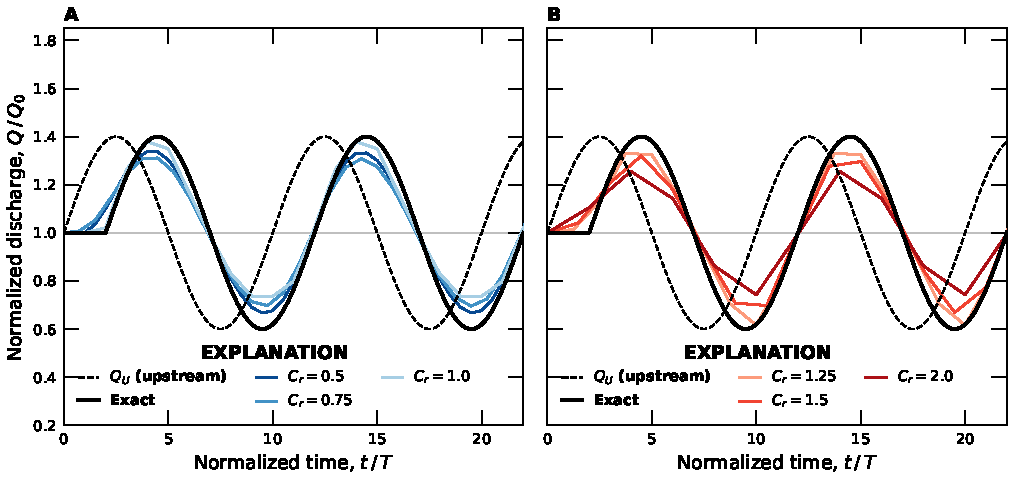
\includegraphics{./Figures/SFRKinematicWave.pdf}
	\caption[Graphs comparing the \mf kinematic-wave scheme against the exact solution at six Courant numbers for a two-reach chain]{Graphs comparing the \mf kinematic-wave finite-difference scheme against the exact kinematic-wave solution at the outlet of a two-reach \mf model (each reach: $\Delta x = 500$ m, $B = 10$ m, $S_0 = 0.001$, $n = 0.03$ s$\,$m$^{-1/3}$) with a sinusoidal upstream boundary condition (eq.~\ref{eqn:sfr-example-qin}) and no lateral inflow. The base flow is $Q_0 = 5$ m$^3$s$^{-1}$, the temporal weighting parameter is $\theta = 1.0$, and time is normalized by the single-reach travel time $T = \Delta x / c_0 \approx 384$ s. The exact solution is delayed by two travel times ($2T$). \textit{A}, Courant numbers $C_r \le 1$ (0.5, 0.75, and 1.0) showing increasing numerical diffusion as $C_r$ decreases from unity; \textit{B}, Courant numbers $C_r > 1$ (1.25, 1.5, and 2.0) showing increasing phase and amplitude errors as the time step coarsens}
	\label{fig:sfr-kinwave}
	\end{center}
\end{figure}

\subsubsection{TVD Results}

The numerical diffusion exhibited by the standard scheme at $C_r < 1$ can be substantially reduced by using the TVD scheme (\texttt{ATS\_COURANT}). To activate the van Leer anti-diffusion correction, a two-reach \mf model is used: the upstream reach is driven by the same sinusoidal inflow (eq.~\ref{eqn:sfr-example-qin}), and the TVD scheme routes the hydrograph through the downstream reach, which has a single upstream neighbor. The exact solution for the two-reach downstream end is the upstream hydrograph delayed by two travel times, $Q_D^\mathrm{exact}(t) = Q_U(t - 2T)$.

Figure~\ref{fig:sfr-kinwave-tvd} compares the standard and TVD schemes against the exact solution at $C_r = 0.5$ (panel~\textit{A}) and $C_r = 0.75$ (panel~\textit{B}). At $C_r = 0.75$ the standard scheme attenuates the peak by 22 percent of the wave amplitude, whereas the TVD scheme, with the van Leer anti-diffusion correction active at the downstream reach, attenuates it by 6 percent and closely tracks the exact solution. At $C_r = 0.5$ the two schemes are nearly indistinguishable, attenuating the peak by 15 and 13 percent, respectively. The benefit of the anti-diffusion correction therefore increases with the Courant number over this range: the standard scheme becomes less accurate as $C_r$ increases toward unity, while the TVD scheme becomes more accurate.

\begin{figure}[!ht]
	\begin{center}
	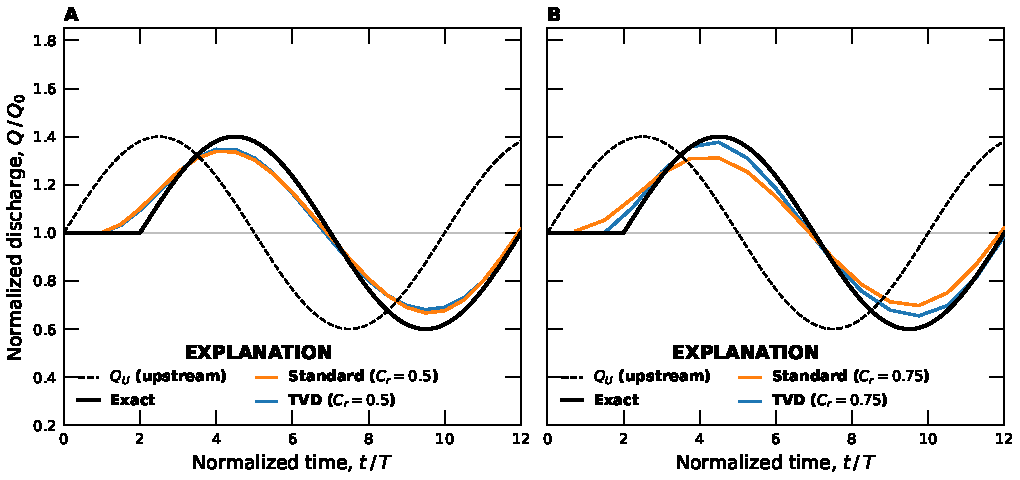
\includegraphics{./Figures/SFRKinematicWaveTVDRouting.pdf}
	\caption[Graphs comparing the \mf standard kinematic-wave and TVD schemes against the exact solution at Courant numbers of 0.5 and 0.75 for a two-reach chain]{Graphs comparing the \mf standard kinematic-wave scheme ($\theta = 1$) and the TVD scheme against the exact kinematic-wave solution for the downstream reach of a two-reach \mf model. Each reach has $\Delta x = 500$ m, $B = 10$ m, $S_0 = 0.001$, $n = 0.03$ s$\,$m$^{-1/3}$, base flow $Q_0 = 5$ m$^3$s$^{-1}$, and the same sinusoidal upstream inflow (eq.~\ref{eqn:sfr-example-qin}). The exact downstream solution is the upstream hydrograph delayed by two travel times. Time is normalized by the single-reach travel time $T \approx 384$ s. \textit{A}, $C_r = 0.5$; \textit{B}, $C_r = 0.75$. At both Courant numbers the standard scheme attenuates the peak, while the TVD scheme closely matches the exact solution}
	\label{fig:sfr-kinwave-tvd}
	\end{center}
\end{figure}

A key advantage of the TVD scheme is that the SFR package budget closes to machine precision at every time step. The standard scheme derives its storage term from the four-point-weighted kinematic-wave residual, so the computed change in stored volume can differ from the actual reach volume change, producing a non-zero budget percent discrepancy. The TVD scheme instead computes the new-time reach volume directly from the explicit volume balance (eq.~\ref{eqn:sfr-tvd-volbal}), guaranteeing exact closure regardless of Courant number or flow conditions.

Figure~\ref{fig:sfr-kinwave-tvd-budget} quantifies this contrast for the same two-reach simulation. At both $C_r = 0.5$ and $C_r = 0.75$, the TVD scheme produces zero percent discrepancy at every time step. The standard scheme produces discrepancies approaching 1 percent, with the largest errors occurring when the sinusoidal inflow gradient is steepest. These are per-step values; because the Newton-Raphson residual changes sign between the rising and falling limbs of the hydrograph, the per-step errors largely cancel over a complete wave cycle and the cumulative volumetric error remains approximately bounded rather than growing with the number of time steps.

\begin{figure}[!ht]
	\begin{center}
	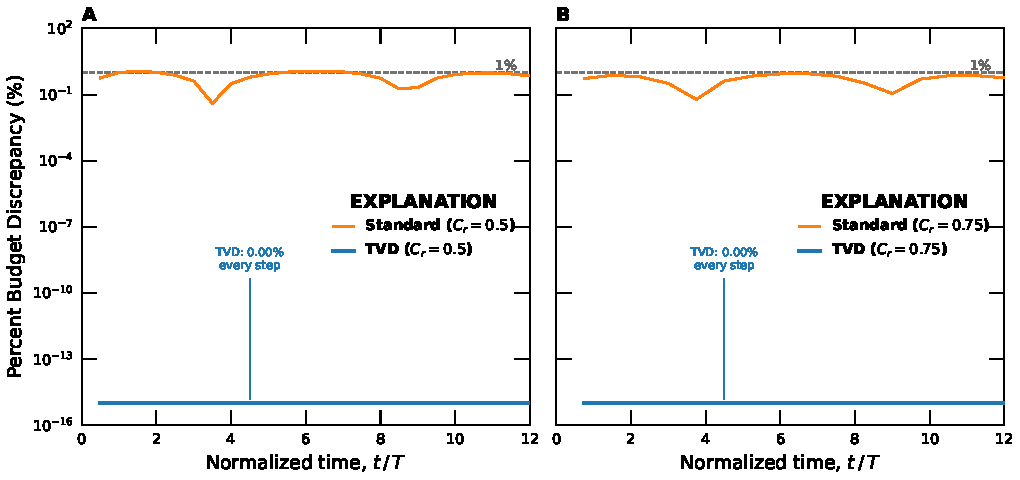
\includegraphics{./Figures/SFRKinematicWaveTVDBudget.pdf}
	\caption[Graphs comparing the per-step SFR budget percent discrepancy of the standard kinematic-wave and TVD schemes at Courant numbers of 0.5 and 0.75]{Graphs comparing the per-step SFR package budget percent discrepancy of the \mf standard kinematic-wave scheme ($\theta = 1$) and the TVD scheme for the same two-reach \mf model shown in figure~\ref{fig:sfr-kinwave-tvd}. Time is normalized by the single-reach travel time $T \approx 384$ s. The discrepancy axis is logarithmic; TVD values at zero are plotted at the floor of the axis. \textit{A}, $C_r = 0.5$; \textit{B}, $C_r = 0.75$. The TVD scheme closes to machine precision at every step; the standard scheme produces discrepancies approaching 1 percent, with the largest values when the flow gradient is steepest}
	\label{fig:sfr-kinwave-tvd-budget}
	\end{center}
\end{figure}

\subsection{Practical Guidance}

\subsubsection{Choosing a Suitable Time Step}
\label{sec:sfr-time-step}

The accuracy of the kinematic-wave scheme depends on the Courant number $C_r = c\,\Delta t / \Delta x$ (eq.~\ref{eqn:sfr-courant}), and figure~\ref{fig:sfr-kinwave} demonstrates that $C_r$ near unity provides the best balance between accuracy and computational efficiency. A practical starting point is therefore to target $C_r \approx 1$ at or near the expected base flow.

For a rectangular channel, the kinematic-wave celerity can be estimated from Manning's equation. When the channel is hydraulically wide (width $B$ much larger than flow depth $d$), the hydraulic radius $R \approx d$, and the celerity simplifies to approximately five thirds of the mean flow velocity $\bar{V} = Q / A$

\begin{equation}
	\label{eqn:sfr-celerity-wide}
	c \approx \frac{5}{3} \bar{V} .
\end{equation}

\noindent Setting $C_r = 1$ and solving for the time step gives the optimal value

\begin{equation}
	\label{eqn:sfr-dt-opt}
	\Delta t_\mathrm{opt} = \frac{\Delta x}{c} \approx \frac{3\,\Delta x\,A_0}{5\,Q_0} ,
\end{equation}

\noindent where $A_0$ and $Q_0$ are the cross-sectional area and discharge at base flow. The optimal time step scales linearly with reach length, so doubling $\Delta x$ doubles $\Delta t_\mathrm{opt}$. Because wave celerity increases with discharge for Manning's-equation channels (equation~\ref{eqn:sfr-celerity-wide}), the Courant number during high-flow conditions will exceed the base-flow value; the code accommodates this automatically by switching to the upstream-only storage stencil (eq.~\ref{eqn:sfr-residual-high-cr}) when $C_r > 1$.

Figure~\ref{fig:sfr-courant} provides two complementary views of the Courant number for a representative rectangular channel ($B = 10$ m, $n = 0.035$). Panel~\textit{A} shows the Courant number $C_r = c\,\Delta t / \Delta x$ evaluated at a reference time step of 10 minutes and reach length of 500 m; for other choices, $C_r$ scales proportionally with $\Delta t$ and inversely with $\Delta x$. The gray band marks the recommended range $0.5 \le C_r \le 2$. As discharge or bed slope increases, the wave celerity rises and the Courant number increases for a fixed time step; steeper and higher-flow reaches require shorter time steps to stay within the acceptable range. Panel~\textit{B} shows the optimal time step $\Delta t_\mathrm{opt} = \Delta x / c$ (minutes) required to achieve $C_r = 1$ for a 500-m reach. The dashed horizontal lines mark common model time steps of 5, 15, and 60 minutes; where a slope curve lies above a reference line, the corresponding time step gives $C_r < 1$ (tends toward excessive diffusion), and where it lies below, the time step gives $C_r > 1$ (tends toward undersampling). The acceptable range spans approximately half to twice the curve value, corresponding to $0.5 \le C_r \le 2$.

When a model contains reaches with different slopes and geometries, the time step should satisfy $C_r \approx 1$ for the reach with the largest celerity-to-length ratio $c / \Delta x$, because all reaches share the same global time step. Courant numbers between approximately 0.5 and 2 are generally acceptable across the network; values outside this range will introduce progressively greater numerical diffusion or phase error (fig.~\ref{fig:sfr-kinwave}).

At the end of each simulation, \mf writes a Courant number summary table to the GWF model listing file. The table reports the minimum, maximum, and mean $C_r$ computed across all transient time steps for each reach; reaches that carried no flow during any transient stress period are reported as~\texttt{--}. The mean is computed over all time steps in which the reach carried flow (dry time steps are excluded). This table provides a direct check on whether the time step kept $C_r$ within the acceptable range throughout the simulation. Equations~\ref{eqn:sfr-celerity-wide} and \ref{eqn:sfr-courant} and figure~\ref{fig:sfr-courant} remain useful for estimating an appropriate time step before the first run. Subdividing unusually long reaches into shorter segments, or merging very short adjacent reaches, can help to equalize Courant numbers across the network and allow a longer global time step.

The \texttt{STORAGE} keyword activates kinematic-wave routing for all reaches in the SFR Package. The option applies only during transient stress periods; steady-state stress periods, including those used to establish initial conditions before a transient simulation, use the standard instantaneous-flow SFR formulation regardless of whether \texttt{STORAGE} is specified, so mixed steady-state and transient simulations are handled automatically.

\begin{figure}[!ht]
	\begin{center}
	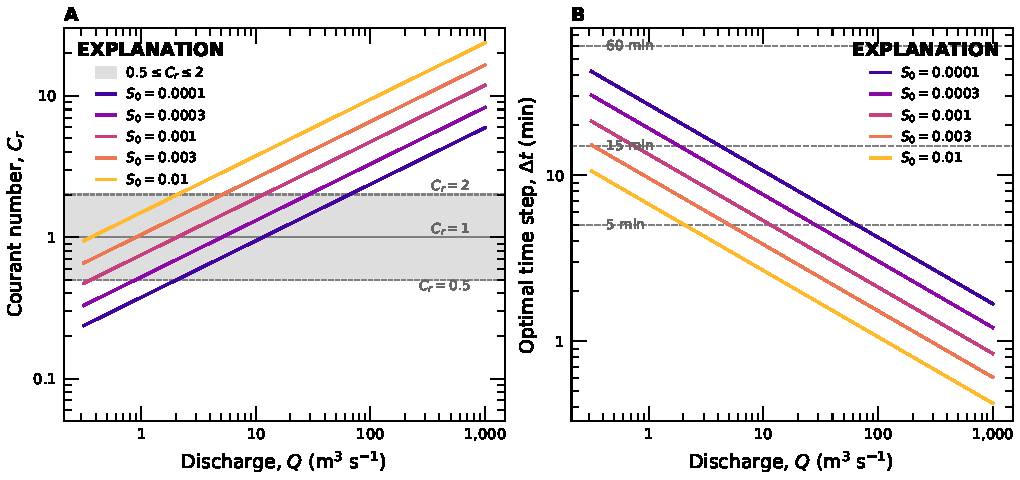
\includegraphics{./Figures/SFRKinematicWaveCourant.pdf}
	\caption[Graphs showing kinematic-wave Courant number and optimal time step as functions of discharge and bed slope]{Graphs showing kinematic-wave routing guidance for a rectangular channel ($B = 10$ m, $n = 0.035$) and reach length of 500 m, as functions of discharge for five bed slopes. Both axes are logarithmic. \textit{A}, Courant number $C_r = c\,\Delta t / \Delta x$ for a reference time step of 10 minutes; $C_r$ scales as $(\Delta t / 10 \text{ min}) \times (500 \text{ m} / \Delta x)$ for other choices. The gray band marks the recommended range $0.5 \le C_r \le 2$; \textit{B}, Optimal time step $\Delta t_\mathrm{opt} = \Delta x / c$ (minutes) for $C_r = 1$. Dashed horizontal lines show common model time steps; where a slope curve lies above a line, that time step gives $C_r < 1$, and where it lies below, $C_r > 1$. The acceptable range is approximately half to twice the curve value}
	\label{fig:sfr-courant}
	\end{center}
\end{figure}

\subsubsection{Applicability Conditions}

The kinematic-wave approximation is most appropriate for steep to moderately sloped, free-draining channels where backwater and inertial effects are negligible. A widely used criterion for assessing applicability is the dimensionless kinematic-wave number \citep{WoolhiserLiggett1967, PonceLiSimons1978}

\begin{equation}
	\label{eqn:sfr-kw-param}
	K = \frac{S_0 \, \Delta x}{F_0^2 \, d_0} ,
\end{equation}

\noindent where $d_0$ is the base-flow depth and $F_0 = \bar{V}_0 / \sqrt{g\,d_0}$ is the Froude number at base flow. Values of $K \gtrsim 10$ indicate that the kinematic wave is a good approximation; values of $K < 5$ suggest that momentum storage, pressure gradients, or backwater effects are important and that the kinematic wave may produce significant errors \citep{Ponce1991}. The kinematic-wave option should not be used in the following situations:

\begin{itemize}

	\item \textit{Very mild slopes} ($S_0 \lesssim 10^{-4}$). Longitudinal pressure gradients and downstream backwater effects become important relative to friction, and the diffusive wave or full dynamic wave is more appropriate.

	\item \textit{Regulated or ponded reaches}. Reaches immediately downstream of dams, weirs, or tidal boundaries are subject to imposed water-surface profiles that invalidate the kinematic assumption.

	\item \textit{Reaches with large and rapidly varying inflow}. Where groundwater seepage substantially alters the flow depth within a reach, the simple celerity estimate may be unreliable and convergence may be slow. Rapidly varying surface inflow has a different effect. Water specified with \texttt{INFLOW} or provided by the MVR Package is added to the reach inflow rather than distributed along the reach, so a runoff event raises the discharge and the celerity together and drives the Courant number up. In a five-reach channel in which a twenty-fold inflow surge raises the Courant number from 0.7 to about 2, the per-step budget discrepancy of the standard scheme rises from below 0.001 percent at base flow to 42 percent, and several time steps are required for it to decay. The TVD scheme closes the budget through the same surge and is the better choice where such events are expected.

	\item \textit{Supercritical or near-critical flow} ($F_0 \gtrsim 1$). The theoretical limit of the kinematic-wave approximation is the onset of roll waves near a Froude number of 2, but the celerity estimate used here (eq.~\ref{eqn:sfr-celerity-wide}) is derived from Manning's equation and becomes less reliable as the flow approaches critical. Reaches with very steep slopes and high velocities may reach or exceed critical conditions at high discharges, and convergence may be slow.

\end{itemize}

\subsubsection{Potential Numerical Problems}

Several numerical issues can arise when using the kinematic-wave option:

\begin{itemize}

	\item \textit{Artificial smoothing of flood peaks} ($C_r \ll 1$). When the time step is much shorter than $\Delta t_\mathrm{opt}$, the numerical scheme introduces an artificial spreading effect---called numerical diffusion---that is not present in the physical system. The result is that computed peak flows at the downstream end of a reach are lower than they should be, and the flood hydrograph appears broader and more rounded: the rising limb rises more gradually, the peak is reduced, and the recession drains more slowly. The wave still translates at roughly the correct speed, but its shape is progressively damped with each time step. Figure~\ref{fig:sfr-kinwave}\textit{A} illustrates this for $C_r = 0.5$ and $C_r = 0.75$: both solutions show the correct timing but underestimate the peak and overestimate the trough relative to the exact solution. Increasing the time step, or subdividing long reaches into shorter segments to reduce $\Delta x$, brings $C_r$ closer to unity and reduces the smoothing.

	\item \textit{Flood-wave timing and peak-flow errors} ($C_r \gg 1$). When the time step is much larger than $\Delta t_\mathrm{opt}$, the scheme takes too few samples of the upstream hydrograph to reconstruct its shape accurately. The practical consequence is that the computed downstream hydrograph can show the flood peak arriving at the wrong time and at the wrong magnitude---peak flows are underestimated and the trough between successive waves is filled in, making the hydrograph appear flatter and more spread out than the true response. The effect worsens as $C_r$ increases beyond 2. Figure~\ref{fig:sfr-kinwave}\textit{B} illustrates this for $C_r = 1.5$ and $C_r = 2$: both solutions preserve the general shape but drift progressively in phase and underestimate the peak. Reducing the time step so that $C_r \lesssim 2$ is recommended; for applications where accurate flood timing or peak-flow magnitude is important, targeting $C_r$ close to 1 is preferable.

	\item \textit{Oscillatory solutions} ($\theta < 1$). The temporal weighting parameter is 1.0 by default, and reducing it below 1 can cause oscillatory solutions at low Courant numbers because the Crank-Nicolson scheme is prone to dispersion errors near $C_r = 0$. The default value $\theta = 1.0$ is strongly recommended for all practical applications.

	\item \textit{Convergence failures on steep wave fronts}. Hydrographs with a very rapid rise---for example, from a sudden change in an upstream boundary condition---can create steep wave fronts that challenge the Newton-Raphson solver (eq.~\ref{eqn:sfr-mf6-update}). Reducing the time step so that the front is better resolved usually resolves the problem.

	\item \textit{Slow convergence with strong groundwater exchange}. The kinematic-wave residual is evaluated within the outer Picard loop that couples stream-aquifer exchange. Reaches with large or rapidly varying leakage fluxes may require more outer iterations to converge. If the model fails to converge within the allowed number of outer iterations, increasing \texttt{OUTER\_MAXIMUM} in the IMS NONLINEAR block or reducing the time step may help.

	\item \textit{Mass-balance drift from discharge flooring}. When the Newton-Raphson update would produce a negligible or negative discharge, the downstream flow is floored at $10^{-30}$~m$^3$\,s$^{-1}$. In reaches that intermittently go dry, repeated flooring can introduce small mass-balance errors. Monitoring the SFR volumetric budget---particularly the storage term---at each time step is recommended to verify that cumulative errors remain small. The TVD scheme (section~\ref{sec:sfr-tvd}) eliminates this source of error by computing the new reach volume directly and reducing the outflow to the available water when the reach would otherwise go dry, guaranteeing exact budget closure by construction at every step.

\end{itemize}
